\documentclass[tikz,border=5pt]{standalone}
\usepackage{pgfplots}\pgfplotsset{compat=1.18}
\definecolor{corba}{HTML}{365FB3}\definecolor{guia}{HTML}{7C3AED}\definecolor{punt}{HTML}{B91C1C}
\begin{document}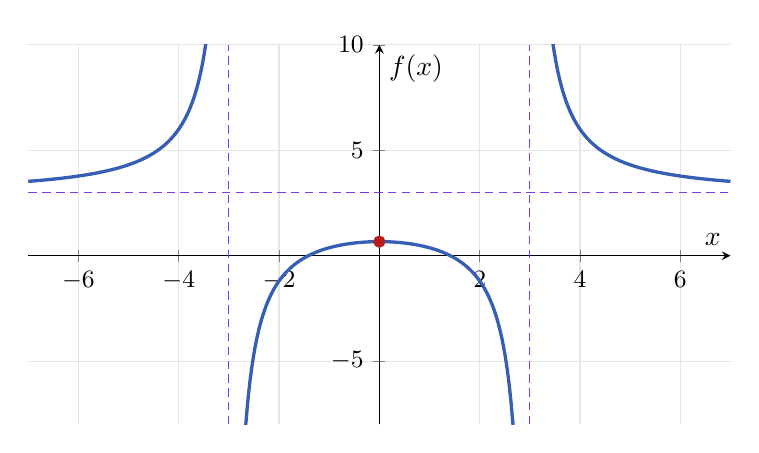
\begin{tikzpicture}
\begin{axis}[width=10.5cm,height=6.4cm,axis lines=middle,xmin=-7,xmax=7,ymin=-8,ymax=10,
 xlabel={$x$},ylabel={$f(x)$},grid=major,grid style={black!10},tick label style={font=\small},samples=160,clip=true]
 \addplot[corba,very thick,domain=-7:-3.04]{(3*x^2-6)/(x^2-9)};\addplot[corba,very thick,domain=-2.96:2.96]{(3*x^2-6)/(x^2-9)};\addplot[corba,very thick,domain=3.04:7]{(3*x^2-6)/(x^2-9)};
 \addplot[guia,densely dashed] coordinates {(-3,-8)(-3,10)};\addplot[guia,densely dashed] coordinates {(3,-8)(3,10)};\addplot[guia,densely dashed,domain=-7:7]{3};
 \addplot[only marks,mark=*,mark size=2pt,punt] coordinates {(0,.6667)};
\end{axis}\end{tikzpicture}\end{document}
